\exercise{Policy Gradient}
In this exercise, you are going to solve the same task of the previous exercise but using policy gradient. 
For the programming exercises, you are allowed to reuse part of the EM code. 
Attach snippets of your code.

\begin{questions}

%----------------------------------------------

\begin{question}{Analytical Derivation}{5}
 	You have a Gaussian policy with diagonal covariance, i.e., $\pi(\vec \theta | \vec \omega) = \gauss{\vec \mu}{ \diag(\vec \sigma^2)}$, where $\vec \omega = [\vec \mu,\vec \sigma]$.
 	Compute analytically the gradient of the logarithm of the policy with respect to the parameters $\vec\omega$, i.e., $\nabla_{\vec\omega} \log \pi(\vec \theta | \vec \omega)$. (Hint: consider the properties of the diagonal covariance matrix.)
\begin{answer}
	 		
	 		\begin{equation}
	 		\nabla_{\vec\omega} \log \pi(\vec \theta | \vec \omega) = \nabla_{\vec\omega} (-log(\sqrt{(2\pi)^k} |diag(\sigma^2)|)-\frac{1}{2} (\theta-\mu)^T diag(\sigma^2)^{-1} (\theta-\mu) )
	 		\end{equation}
	 		
	\begin{equation}
	\nabla_{\vec\omega} \log \pi(\vec \theta | \vec \omega) = \nabla_{\vec\omega} (-log(\sqrt{(2\pi)^k} (\sigma^{2k}))-\frac{1}{2 \sigma^2} \sum_{i=1}^k (\theta_i - \mu_i)^2)
	\end{equation}
	
\begin{equation}
\nabla_{\vec\omega} \log \pi(\vec \theta | \vec \omega) = \begin{bmatrix}
\frac{\partial}{\partial \mu}\log \pi(\vec \theta | \vec \omega)\\\frac{\partial}{\partial \sigma}\log \pi(\vec \theta | \vec \omega)
\end{bmatrix}
\end{equation}

\begin{equation}
\frac{\partial}{\partial \mu}\log \pi(\vec \theta | \vec \omega)=\frac{1}{\sigma^2} \sum_{i=1}^{k}(\theta_i - \mu_i)
\end{equation}

\begin{equation}
\frac{\partial}{\partial \sigma}\log \pi(\vec \theta | \vec \omega)=-\frac{2k}{\sigma}+\frac{1}{\sigma^3} \sum_{i=1}^{k}(\theta_i - \mu_i)^2
\end{equation}

Note that:
 	 		\begin{equation}
 	 		\gauss{\vec \mu}{ \diag(\vec \sigma^2)}=\frac{1}{\sqrt{(2\pi)^k} |diag(\sigma^2)|} exp(-0.5 (\theta-\mu)^T diag(\sigma^2)^{-1} (\theta-\mu))
 	 		\end{equation}	 	
 		
 	\begin{equation}
(\theta-\mu)^T diag(\sigma^2)^{-1} (\theta-\mu) = \frac{1}{\sigma^2} \sum_{i=1}^k (\theta_i - \mu_i)^2
  \end{equation}

	\end{answer}

\end{question}

%----------------------------------------------

\begin{question}{Programming Exercise}{5}
	Consider the same robotic task as in the previous exercise and this time solve it with policy gradient. 
	Use an initial mean of $\vec \mu_0 = [0 \dots 0]$ and a fixed $\vec \sigma = \diag([10 \dots 10])$ (i.e., do \textbf{not} update $\vec\sigma$). Set the learning rate to $\alpha=0.1$ and use the same hyperparameters as before (25 episodes sampled for each iteration and max 100 iterations).\\
	Repeat the learning 10 times and plot the mean of the average return of all runs with $95\%$ confidence.
	Use the logarithmic scale for your plot. Comment your results.
	
	\begin{answer}
	\begin{equation}
		\omega_{k+1}=\omega_k + \alpha \nabla_{\omega} J_{\omega}
	\end{equation}
Update rule for $\theta$:
		\begin{equation}
		\sigma_{k+1}=\sigma_k + \alpha \frac{\partial}{\partial \sigma} J({\sigma_k})
		\end{equation}
		
		Update rule for $\mu$:
		\begin{equation}
		\mu_{k+1}=\mu_k + \alpha \frac{\partial}{\partial \mu}  J({\mu_k})
		\end{equation}



TODO PLOT HERE
	\end{answer}
\end{question}


%----------------------------------------------


\begin{question}{A Little Trick}{5}
	How would you improve the above implementation? (Beside using a smaller or adaptive learning rate, or using the natural gradient). What is the theory behind this ``trick''? Repeat the learning and discuss the results.
	
	\begin{answer}
	\begin{equation}
	\nabla_\omega J_\omega \sum_{i=1}^{N} \nabla_\omega log \pi (\theta; \omega)(R_i - b)
	\end{equation}
		
	The baseline has to be subtracted. Thereby the possibly high gradient of the variance can be reduced. It is still unbiased.
	
	\begin{center}
		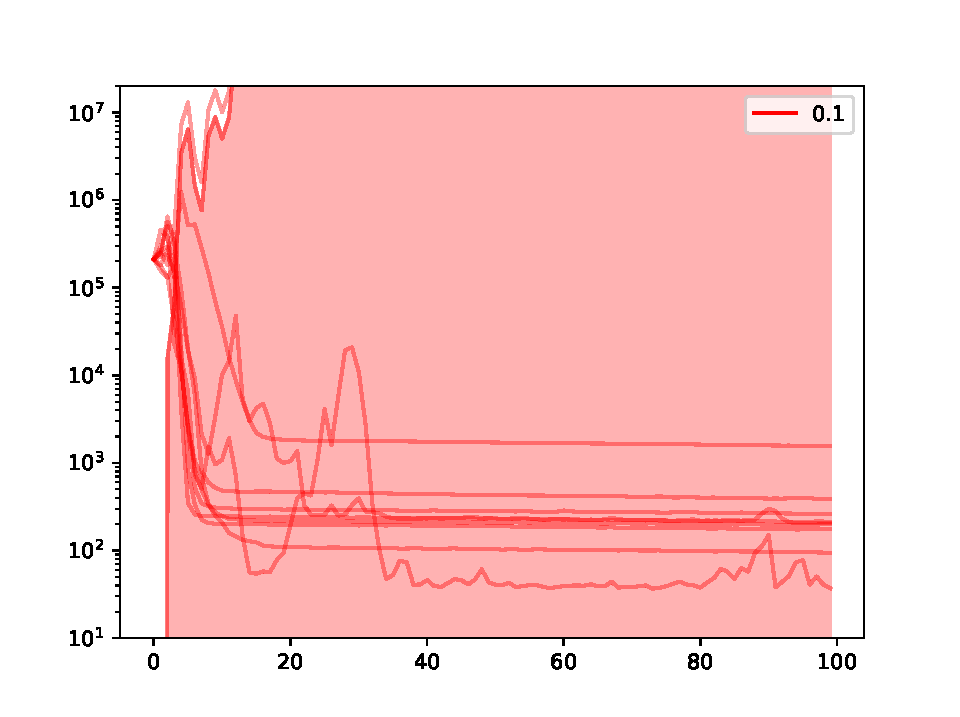
\includegraphics[width=0.5\textwidth]{img/PG-c.pdf}
		\captionof{figure}{The average return over the episodes of for $\lambda=0.1$ with baseline subtracted of the PG algorithm}
	\end{center}
	
	\end{answer}

\end{question}
	

%----------------------------------------------

\begin{question}{Learning Rate}{5}
	Repeat the optimization changing the learning rate to $\alpha=0.4$ and $\alpha = 0.2$ (keep the trick of the previous exercise).
	Plot in one figure the mean of the average returns for all $\alpha$ with $95\%$ confidence.
	How does the value of $\alpha$ affect the convergence of the algorithm? 
	Use the logarithmic scale for your plot.
		
\begin{answer}
The higher the $\alpha$ the faster the algorithm converges.

	\begin{center}
		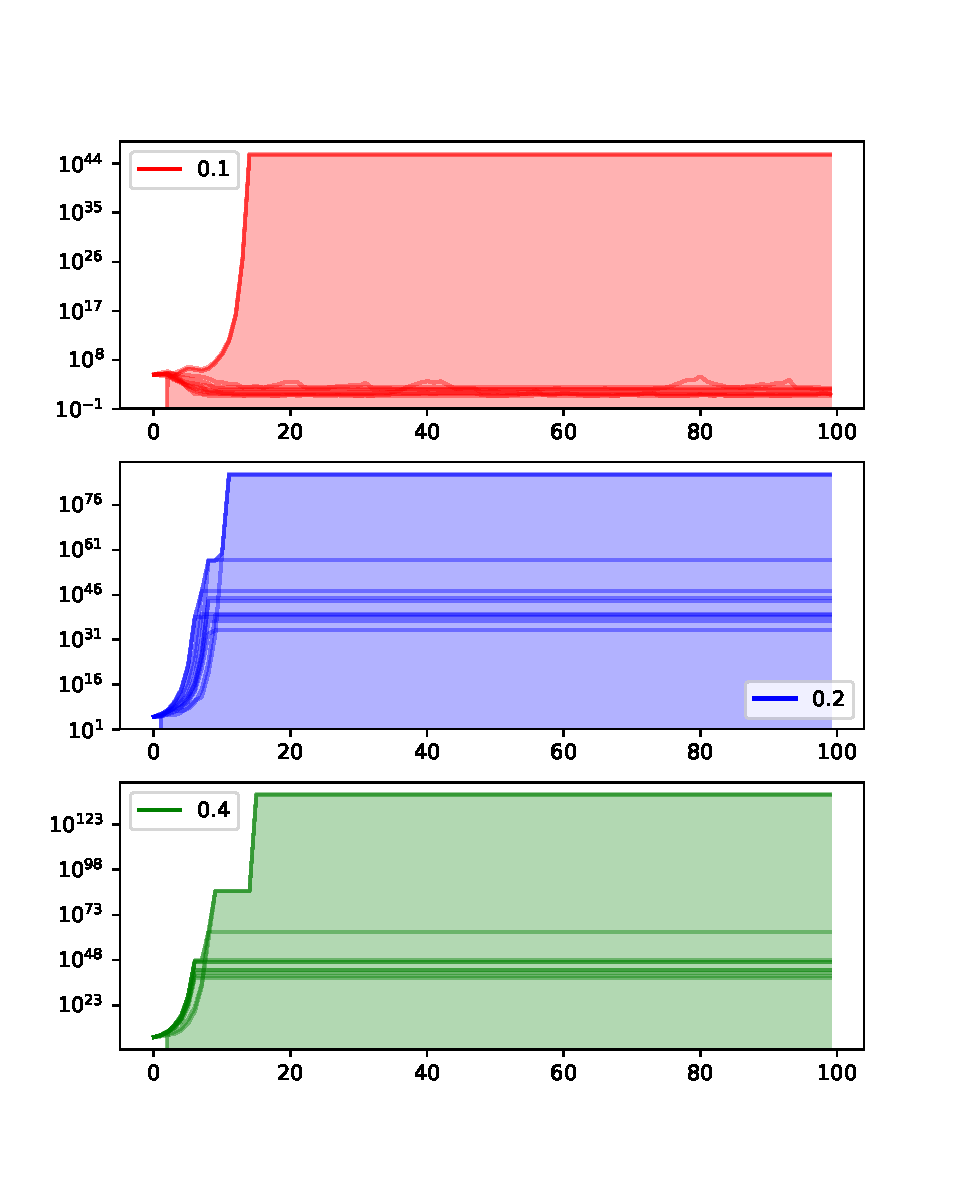
\includegraphics[width=0.5\textwidth]{img/PG-d.pdf}
		\captionof{figure}{The average return over the episodes for different learning rates $\alpha$ }
	\end{center}
\end{answer}
\end{question}

%----------------------------------------------
	
\begin{question}{Variable Variance}{5}
	Try to improve the optimization process by learning also the variance $\vec \sigma$. Is it easier or harder to learn also the variance? Why?
	\\Without using the natural gradient, tune the learning process to \textbf{achieve better results}. If you think it is necessary, you can impose a lower bound to avoid that the variance collapses to infinitely small values (e.g., if $\sigma(i)<\sigma_{\text{lower}}$ then $\sigma(i) = \sigma_{\text{lower}}$).
	In one figure, plot the learning trend with confidence interval as done before and compare it to the one achieved with $\alpha = 0.4$ before.
	
\begin{answer}
	Now use:
\begin{equation}
\sigma_{k+1}=\sigma_k + \alpha \frac{\partial}{\partial \omega} J({\sigma_k})
\end{equation}
% Füge update rule für sigma ein.
\end{answer}

\end{question}

%----------------------------------------------

	
\begin{question}[bonus]{Natural Gradient}{5}
	Write down the equation of the natural gradient. What is the theory behind it?
	Is it always easy to use?
	
\begin{answer}
The Natural Gradient: (with G the Fischer Information Matrix)
\begin{equation}
	\nabla_\omega J = G(\omega)^{-1} \nabla_\omega J
\end{equation}
Theory of the Natural Gradient:\\
KL divergence is a measure of how close a distribution is to another distribution.This brings us to the natural gradient. If we blindly update our network in the direction of its gradients, there are no guarantees the distribution of the new network will be similar to the old one.

To fix this, we first consider all combinations of parameters that result in a new network a constant KL divergence away from the old network. This constant value can be viewed as the step size or learning rate. Out of all these possible combinations, we choose the one that minimizes our loss function.

Basically, we're adding in a constraint to our update, that the new network will behave relatively similar to our old one. Our step size corresponds directly to the actual distribution of the network, not it's parameter's values.

This comes with the added benefit of a more stable learning process. Especially when we're updating using a randomly sampled batch, some outliers may make drastic changes to a network's parameters. With natural gradient descent, a single update can't make too much of an impact. 
	
Note that: Replacing a sigmoid activation with a tanh function would change the standard gradient, but not the natural gradient. 

Is it always easy to use:
No actually NG is much more computationally expensive compared to the simple gradient. Moreover there are two types of KL:
\begin{itemize}
	\item Moment projection
	\item Information projection (is not unique selects the mode!)
\end{itemize}

It is not so easy to select which KL should be used.

Note that KL can be approximated by the FIM which captures information how the single parameters influence the distribution.


\end{answer}
\end{question}

\end{questions}